\documentclass[10pt,a4paper]{article}
\usepackage{amsmath}
\usepackage{amssymb}
\usepackage{booktabs}
\usepackage{tabularx}
\usepackage{geometry}
\geometry{margin=0.6in,top=0.5in,bottom=0.5in}
\usepackage{enumitem}
\usepackage{siunitx}
\usepackage{tikz}
\usepackage{xcolor}
\usepackage{multicol}
\usetikzlibrary{calc,arrows.meta}
\setlength{\parindent}{0pt}
\setlength{\parskip}{0.3em}

% Vector notation
\newcommand{\vv}[1]{\vec{#1}}
\newcommand{\magn}[1]{|#1|}

% TikZ styles for vector diagrams
\colorlet{vec_f1}{blue!80!black}
\colorlet{vec_f2}{red!80!black}
\colorlet{vec_fr}{green!60!black}
\colorlet{vec_translated}{gray!60}
\tikzset{
    vector/.style={-{Stealth[length=2.5mm,width=1.5mm]},thick},
    vector_translated/.style={-{Stealth[length=1.5mm,width=1mm]},dashed,thin},
}

\begin{document}
\begin{center}
\textbf{\large Engineering Calculation Report: Problem 2-1}\\[0.3em]
\small Generated: {{GENERATED_DATE}}
\end{center}
\vspace{-0.5em}
\hrule
\vspace{0.5em}

\textbf{\underline{Problem Setup}}\\[0.5em]
\noindent
\begin{minipage}[c]{0.32\textwidth}
\begin{center}
\begin{tabular}{lSSl}
\toprule
Vector & {$\magn{\vv{F}}$ (N)} & {$\theta$ (deg)} & Ref \\
\midrule
$\vv{F_1}$ & 450.0 & 60.0 & $+x$ \\
$\vv{F_2}$ & 700.0 & 15.0 & $-x$ \\
\midrule
$\vv{F_R}$ & ? & ? & $+x$ \\
\bottomrule
\end{tabular}
\end{center}
\end{minipage}%
\hfill
\begin{minipage}[c]{0.66\textwidth}
\begin{center}

\begin{tikzpicture}[scale=0.55,baseline=(current bounding box.north)]
  \coordinate (A) at (0.000,0.000);
  \coordinate (B) at (1.498,2.595);
  \coordinate (C) at (-4.502,-1.206);
  \coordinate (D) at (-3.004,1.388);
  \draw[->,gray] (0.000,0.000) -- (4.661,0.000) node[right] {$+x$};
  \draw[->,gray] (0.000,0.000) -- (-4.661,0.000) node[left] {$-x$};
  \draw[->,gray] (0.000,0.000) -- (0.000,4.661) node[above] {$+y$};
  \draw[->,gray] (0.000,0.000) -- (0.000,-4.661) node[below] {$-y$};
  % Draw parallelogram sides (translated vectors - dashed)
  \draw[vector_translated,vec_translated] (B) -- (D);
  \draw[vector_translated,vec_translated] (C) -- (D);
  % Draw main vectors
  \draw[vector,vec_f1] (A) -- (B) node[above right,pos=1] {$\vv{F_1} = 450\,\text{N}$};
  \draw[vector,vec_f2] (A) -- (C) node[below left,pos=1] {$\vv{F_2} = 700\,\text{N}$};
  \draw[vector,vec_fr] (A) -- (D) node[above left,pos=1] {$\vv{F_R}$};
  \draw[vec_f1,thin] (0.000,0.000) ++(0:1.631) arc (0:59.99999999999999:1.631);
  \node[vec_f1,anchor=west] at (1.716,0.991) {$60^\circ$};
  \draw[vec_f2,thin] (0.000,0.000) ++(180:2.330) arc (180:195.0:2.330);
  \node[vec_f2,anchor=east] at (-2.657,-0.350) {$15^\circ$};
  \fill (A) circle (2pt) node[below left] {$O$};
\end{tikzpicture}
\end{center}
\end{minipage}

\vspace{0.5em}

\textbf{\underline{Equations Used}}\\[0.5em]
\hspace*{1em}(1) $\displaystyle \magn{\vv{F_R}}^2 = \magn{\vv{F_1}}^2 + \magn{\vv{F_2}}^2 - 2 \cdot \magn{\vv{F_1}} \cdot \magn{\vv{F_2}} \cdot \cos(\angle(\vv{F_1}, \vv{F_2}))$\\[0.5em]
\hspace*{1em}(2) $\displaystyle \frac{\sin(\angle(\vv{F_1}, \vv{F_R}))}{\magn{\vv{F_2}}} = \frac{\sin(\angle(\vv{F_1}, \vv{F_2}))}{\magn{\vv{F_R}}}$


\vspace{0.5em}
\textbf{\underline{Solution}}\\[0.5em]
\hspace*{1em}\textbf{Step 1:} $\angle(\vv{F_1}, \vv{F_2})$\\[0.2em]
\hspace*{2em}$\angle(\vv{F_1}, \vv{F_2}) = \magn{\angle(\vv{x}, \vv{F_1}) - \angle(\vv{-x}, \vv{F_2})} = \magn{60^{\circ} - 15^{\circ}} = 45^{\circ}$\\[0.3em]
\hspace*{1em}\textbf{Step 2:} $\magn{\vv{F_R}}$ using Eq 1\\[0.2em]
\hspace*{2em}$\magn{\vv{F_R}} = \sqrt{(450.0\ \text{N})^2 + (700.0\ \text{N})^2 - 2(450.0\ \text{N})(700.0\ \text{N})\cos(45.0^{\circ})} = 497.0\ \text{N}$\\[0.3em]
\hspace*{1em}\textbf{Step 3:} $\angle(\vv{F_1}, \vv{F_R})$ using Eq 2\\[0.2em]
\hspace*{2em}$\angle(\vv{F_1}, \vv{F_R}) = \sin^{-1}(700.0\ \text{N} \cdot \frac{\sin(45.0^{\circ})}{497.0\ \text{N}}) = 95.2^{\circ}$\\[0.3em]
\hspace*{1em}\textbf{Step 4:} $\angle(\vv{x}, \vv{F_R})$ with respect to +x\\[0.2em]
\hspace*{2em}$\angle(\vv{x}, \vv{F_R}) = \angle(\vv{x}, \vv{F_1}) + \angle(\vv{F_1}, \vv{F_R}) = 60.0^{\circ} + 95.2^{\circ} = 155.2^{\circ}$

\vspace{0.5em}
\textbf{\underline{Results}}\\[0.5em]
\noindent
\begin{minipage}[c]{0.32\textwidth}
\begin{center}
\begin{tabular}{lSSl}
\toprule
Vector & {$\magn{\vv{F}}$ (N)} & {$\theta$ (deg)} & Ref \\
\midrule
$\vv{F_R}$ & 497.0 & 155.2 & $+x$ \\
\bottomrule
\end{tabular}
\end{center}
\end{minipage}%
\hfill
\begin{minipage}[c]{0.66\textwidth}
\begin{center}

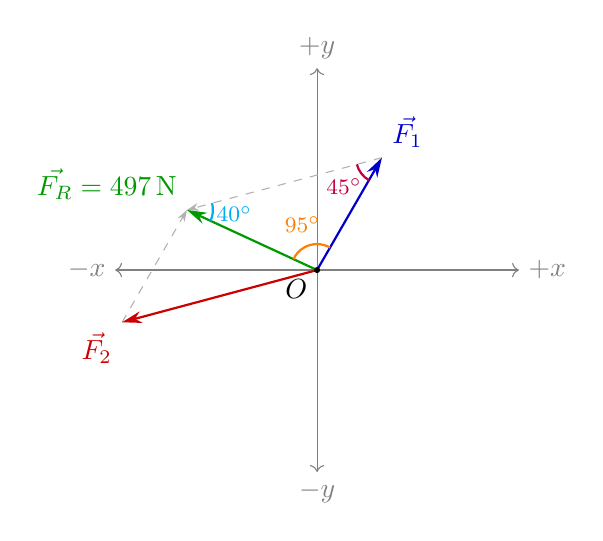
\begin{tikzpicture}[scale=0.55,baseline=(current bounding box.north)]
  \coordinate (A) at (0.000,0.000);
  \coordinate (B) at (1.498,2.595);
  \coordinate (C) at (-4.502,-1.206);
  \coordinate (D) at (-3.004,1.388);
  \draw[->,gray] (0.000,0.000) -- (4.661,0.000) node[right] {$+x$};
  \draw[->,gray] (0.000,0.000) -- (-4.661,0.000) node[left] {$-x$};
  \draw[->,gray] (0.000,0.000) -- (0.000,4.661) node[above] {$+y$};
  \draw[->,gray] (0.000,0.000) -- (0.000,-4.661) node[below] {$-y$};
  \draw[vector_translated,vec_translated] (B) -- (D);
  \draw[vector_translated,vec_translated] (C) -- (D);
  \draw[vector,vec_f1] (A) -- (B) node[above right,pos=1] {$\vv{F_1}$};
  \draw[vector,vec_f2] (A) -- (C) node[below left,pos=1] {$\vv{F_2}$};
  \draw[vector,vec_fr] (A) -- (D) node[above left,pos=1] {$\vv{F_R} = 497\,\text{N}$};
  \draw[orange,thick] (0.000,0.000) ++(60.0:0.600) arc (60.0:155.2:0.600);
  \node[orange,font=\footnotesize] at (-0.333,1.049) {$95^\circ$};
  \draw[purple,thick] (1.498,2.595) ++(195.0:0.600) arc (195.0:240.0:0.600);
  \node[purple,font=\footnotesize] at (0.625,1.925) {$45^\circ$};
  \draw[cyan,thick] (-3.004,1.388) ++(335.2:0.600) arc (335.2:375.0:0.600);
  \node[cyan,font=\footnotesize] at (-1.908,1.294) {$40^\circ$};
  \fill (A) circle (2pt) node[below left] {$O$};
\end{tikzpicture}
\end{center}
\end{minipage}

\vspace{0.5em}
\hrule
\vspace{0.3em}
\begin{center}
\footnotesize
\textbf{Signatures:} Calc. By: \rule{2cm}{0.4pt} \quad Rev. By: \rule{2cm}{0.4pt} \quad Appr. By: \rule{2cm}{0.4pt}
\vspace{0.3em}

\scriptsize\textit{Generated by Qnty Library (Beta). Independent verification required. Users assume full responsibility.}
\end{center}
\end{document}